\section{Algorytm}
\label{ch:algorytm}
Celem algorytmu jest odtworzenia poprawnego sygnału $u$ z zarejestrowanego przebiegu $v = u + g$, gdzie $g$ jest addytywnym szumem. Dla podanej próbki sygnału $s$ estymata  $\hat{u}\left ( s \right )$ stanowi sumę ważoną innych próbek $t$ które zawierają się w sąsiedztwie $N(s)$ 


\begin{equation}
\label{eq:jeden}
\hat{u}\left(s\right)= \frac{1}{Z(s)} \sum_{t\in N(s)} w(s,t)v(t)
\end{equation}

gdzie $Z(s) = \sum_{t} w(s,t)$, a waga dla próbki wynosi $w$:

\begin{equation}
\label{eq:dwa}
w(s,t)= \textup{exp} \left (  -\frac{\sum_{\delta \in \Delta }{(v(s+\delta)-v(t+\delta))^{2}}}{2L_{\Delta}\lambda^{2}}\right ) \equiv \textup{exp} \left ( -\frac{d^{2}(s,t)}{2L_{\Delta}\lambda^{2}}\right )
\end{equation}

W równaniu (\ref{eq:dwa}) $\lambda$ jest parametrem opisującym pasmo, podczas gdy $\Delta$ reprezentuje lokalny fragment próbek wokół punktu $s$, zawierający $L_{\Delta}$ próbek. Okolice punktu $t$ są analizowane wycinkiem o tym samym kształcie.

Należy zwrócić uwagę, że $w(s,s)=1$. Stosując metodą NLM dla zaszumionych obrazów, często zakłada się, że:
\begin{equation}
\label{eq:trzy}
w(s,s) = \max_{t\in N(s),t\neq s}w(s,t)
\end{equation}
W przypadku odszumiania sygnału EKG, stosując powyższą korektę dochodzi do nadmiernego gładzenia niektórych zespołów QRS, co widoczne jest na rysunku \ref{rys:rzekomapoprawa}. Pozostano więc przy oryginalnej wadze  $w(s,s)=1$.
\begin{figure}[!htb]
	\begin{center}
		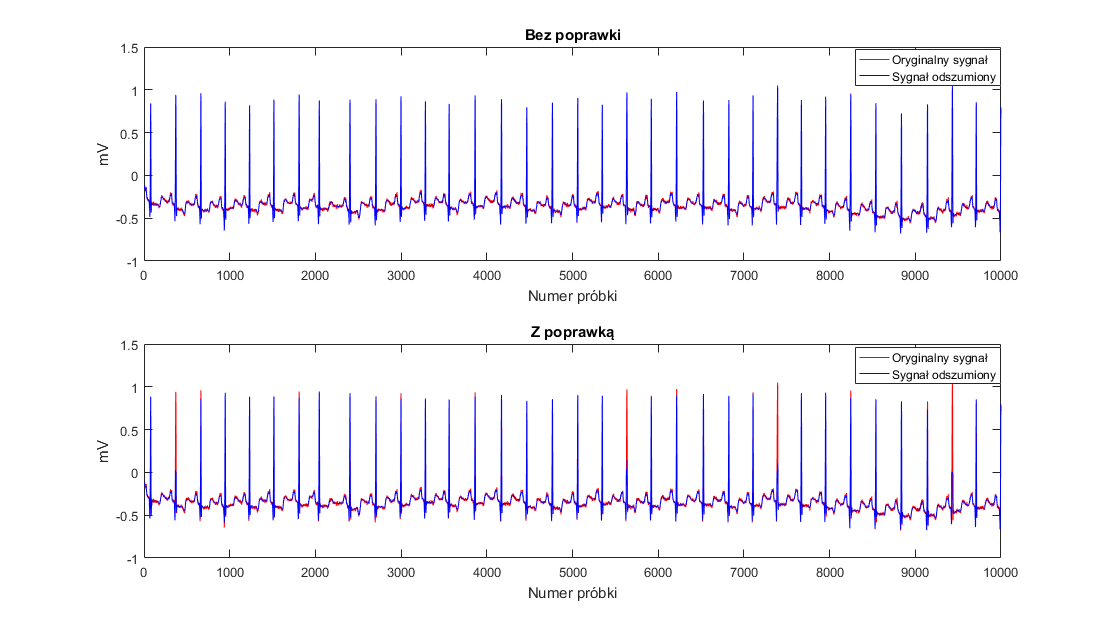
\includegraphics[width=15cm,clip]
		{img/rzekomapoprawa.png}
	\end{center}
	\caption{Sprawdzenie wprowadzenia korekty opisanej wzorem \ref{eq:trzy}. Wprowadzona poprawka tak naprawdę pogarsza estymatę oryginalnego sygnału EKG.}
	\label{rys:rzekomapoprawa}
\end{figure}

Cechą odróżniającą metodę NLM są wagi $w(s,t)$ które zależą od podobieństwa między fragmentami, a nie odległością między punktami $s$ i $t$. Uśrednianie podobnych fragmentów pozwala na znacznie lepsze  zachowanie zboczy sygnału niż inne typowe filtry (np. Gaussowski, dolnoprzepustowy).  Biorąc pod uwagę że podobieństwo między fragmentami jest widoczne na całym przebiegu, może on być uznany za sąsiedztwo badanego fragmentu. Taki zabieg powoduje że proces jest całkowicie nielokalny.\cite{tracey2012nonlocal}

